
\documentclass[a4paper,11pt]{article}
\usepackage[a4paper, margin=8em]{geometry}

% usa i pacchetti per la scrittura in italiano
\usepackage[french,italian]{babel}
\usepackage[T1]{fontenc}
\usepackage[utf8]{inputenc}
\frenchspacing 

% usa i pacchetti per la formattazione matematica
\usepackage{amsmath, amssymb, amsthm, amsfonts}

% usa altri pacchetti
\usepackage{gensymb}
\usepackage{hyperref}
\usepackage{standalone}

% imposta il titolo
\title{Appunti Fondamenti di Automatica}
\author{Luca Seggiani}
\date{2025}

% disegni
\usepackage{pgfplots}
\pgfplotsset{width=10cm,compat=1.9}

% imposta lo stile
% usa helvetica
\usepackage[scaled]{helvet}
% usa palatino
\usepackage{palatino}
% usa un font monospazio guardabile
\usepackage{lmodern}

% tikz in sans
\tikzset{every picture/.style={/utils/exec={\sffamily}}}

\renewcommand{\rmdefault}{ppl}
\renewcommand{\sfdefault}{phv}
\renewcommand{\ttdefault}{lmtt}

% circuiti
\usepackage{circuitikz}
\usetikzlibrary{babel}

% disponi il titolo
\makeatletter
\renewcommand{\maketitle} {
	\begin{center} 
		\begin{minipage}[t]{.8\textwidth}
			\textsf{\huge\bfseries \@title} 
		\end{minipage}%
		\begin{minipage}[t]{.2\textwidth}
			\raggedleft \vspace{-1.65em}
			\textsf{\small \@author} \vfill
			\textsf{\small \@date}
		\end{minipage}
		\par
	\end{center}

	\thispagestyle{empty}
	\pagestyle{fancy}
}
\makeatother

% disponi teoremi
\usepackage{tcolorbox}
\newtcolorbox[auto counter, number within=section]{theorem}[2][]{%
	colback=blue!10, 
	colframe=blue!40!black, 
	sharp corners=northwest,
	fonttitle=\sffamily\bfseries, 
	title=Teorema~\thetcbcounter: #2, 
	#1
}

% disponi definizioni
\newtcolorbox[auto counter, number within=section]{definition}[2][]{%
	colback=red!10,
	colframe=red!40!black,
	sharp corners=northwest,
	fonttitle=\sffamily\bfseries,
	title=Definizione~\thetcbcounter: #2,
	#1
}

% disponi problemi
\newtcolorbox[auto counter, number within=section]{problem}[2][]{%
	colback=green!10,
	colframe=green!40!black,
	sharp corners=northwest,
	fonttitle=\sffamily\bfseries,
	title=Problema~\thetcbcounter: #2,
	#1
}

% disponi codice
\usepackage{listings}
\usepackage[table]{xcolor}

\lstdefinestyle{codestyle}{
		backgroundcolor=\color{black!5}, 
		commentstyle=\color{codegreen},
		keywordstyle=\bfseries\color{magenta},
		numberstyle=\sffamily\tiny\color{black!60},
		stringstyle=\color{green!50!black},
		basicstyle=\ttfamily\footnotesize,
		breakatwhitespace=false,         
		breaklines=true,                 
		captionpos=b,                    
		keepspaces=true,                 
		numbers=left,                    
		numbersep=5pt,                  
		showspaces=false,                
		showstringspaces=false,
		showtabs=false,                  
		tabsize=2
}

\lstdefinestyle{shellstyle}{
		backgroundcolor=\color{black!5}, 
		basicstyle=\ttfamily\footnotesize\color{black}, 
		commentstyle=\color{black}, 
		keywordstyle=\color{black},
		numberstyle=\color{black!5},
		stringstyle=\color{black}, 
		showspaces=false,
		showstringspaces=false, 
		showtabs=false, 
		tabsize=2, 
		numbers=none, 
		breaklines=true
}

\lstdefinelanguage{javascript}{
	keywords={typeof, new, true, false, catch, function, return, null, catch, switch, var, if, in, while, do, else, case, break},
	keywordstyle=\color{blue}\bfseries,
	ndkeywords={class, export, boolean, throw, implements, import, this},
	ndkeywordstyle=\color{darkgray}\bfseries,
	identifierstyle=\color{black},
	sensitive=false,
	comment=[l]{//},
	morecomment=[s]{/*}{*/},
	commentstyle=\color{purple}\ttfamily,
	stringstyle=\color{red}\ttfamily,
	morestring=[b]',
	morestring=[b]"
}

% disponi sezioni
\usepackage{titlesec}

\titleformat{\section}
	{\sffamily\Large\bfseries} 
	{\thesection}{1em}{} 
\titleformat{\subsection}
	{\sffamily\large\bfseries}   
	{\thesubsection}{1em}{} 
\titleformat{\subsubsection}
	{\sffamily\normalsize\bfseries} 
	{\thesubsubsection}{1em}{}

% disponi alberi
\usepackage{forest}

\forestset{
	rectstyle/.style={
		for tree={rectangle,draw,font=\large\sffamily}
	},
	roundstyle/.style={
		for tree={circle,draw,font=\large}
	}
}

% disponi algoritmi
\usepackage{algorithm}
\usepackage{algorithmic}
\makeatletter
\renewcommand{\ALG@name}{Algoritmo}
\makeatother

% disponi numeri di pagina
\usepackage{fancyhdr}
\fancyhf{} 
\fancyfoot[L]{\sffamily{\thepage}}

\makeatletter
\fancyhead[L]{\raisebox{1ex}[0pt][0pt]{\sffamily{\@title \ \@date}}} 
\fancyhead[R]{\raisebox{1ex}[0pt][0pt]{\sffamily{\@author}}}
\makeatother

\begin{document}

% sezione (data)
\section{Lezione del 16-05-25}

% stili pagina
\thispagestyle{empty}
\pagestyle{fancy}

% testo
\subsection{Controllori PID}
Una classe di regolatori standard è quella rappresentata dai controllori \textbf{PID}, \textit{Proporzionale Integrale Derivata}.

Questi implementano effettivamente la funzione:
$$
u(t) = K\left( e(t) + \frac{1}{T_i} \int_0^t e(\tau) \, d\tau + T_d \frac{d \, e(t)}{dt} \right)
$$
cioè in dominio di Laplace:
$$
R(s) = K_P + \frac{K_I}{s} + K_D(s)
$$
posto:
$$
K_P = K, \quad K_I = \frac{K}{T_i}, \quad K_D = K \cdot T_d
$$

Se ne possono implementare anche le versioni P e PI.
Il $95\%$ dei controllori industriali sono di questo tipo.

Una forma più standard del PID si ottiene come:
$$
R(s) = K_P + \frac{K_I}{s} + K_D(s) = \frac{K_D s^2 + K_P s + K_I}{s}
$$
$$
= K_P\left( 1 + \frac{1}{T_I s} + T_D s \right) = K_P \frac{T_I T_D s^2 + T_I s + 1}{T_I s}
$$

Una cosa che dovrebbe saltare all'occhio è che il termine derivata introduce uno zero instabile, cioè uno zero in più di quanti poli abbiamo.
Questo significherà che i PID implementati nella realtà avranno necessariamente un polo in più ad alta frequenza, che possiamo intendere come termine "filtratore" della derivata.

Nei PID digitali, questa pulsazione massima è legata alla frequenza di campionamento massimo del dispositivo.

Continuiamo comunque a trattare, almeno dal punto di vista matematico, la forma del PID ideale.

Un regolatore PID ha quindi funzione di trasferimento con un polo all'origine e 2 zeri:
$$
z_{1, 2} = \frac{- T_I \pm \sqrt{T_I(T_I - 4 T_D)}}{2 T_I T_D}
$$

Qualitativamente, il polo nell'origine garantisce prestazioni di precisione a regime, mentre gli zeri permettono di recuperare fase e, assieme alla costante di guadagno, di soddisfare le specifiche di transitorio.

La disponibilità del modello a controllore PID consente da un lato di poter usare una struttura standard per il controllo, mentre dall'altro diminuisce i gradi di libertà nel progetto del controllore.

\subsubsection{Montaggio di un PID e filtraggio della derivata}
Il montaggio classico dei PID consiste nell'avere la semplice somma dei 3 termini:
\begin{center}
	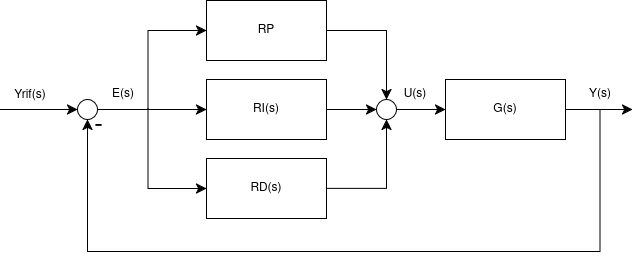
\includegraphics[scale=0.5]{../figures/pid.png}
\end{center}

In questa configurazione, però, l'azione derivativa sul segnale di errore può causare segnali di controllo a frequenza molto elevata (e probabilmente instabilità).
Potremmo pensare di risolvere questo problema inserendo un filtro passa basso sul riferimento $Y_{rif}(s)$:
\begin{center}
	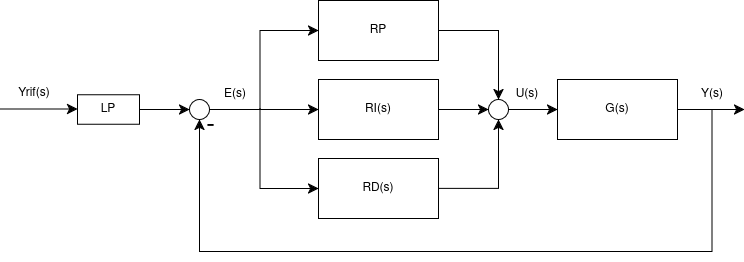
\includegraphics[scale=0.5]{../figures/pid_filt.png}
\end{center}

Un montaggio alternativo, e più conveniente, è quello che deriva direttamente l'uscita e la spedisce negata al sistema:
\begin{center}
	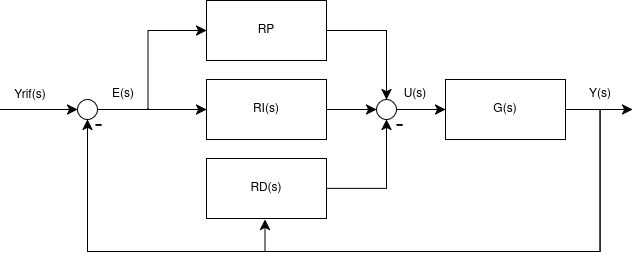
\includegraphics[scale=0.5]{../figures/pid_deriv.png}
\end{center}
Questo viene naturale sfruttando che, per $Y_{rif}'(s)$ probabilmente nullo o comunque che si vuole trascurare, si ha:
$$
E(s) = Y_{rif}(s) - Y(s) \implies E'(s) = Y_{rif}'(s) - Y'(s) \approx - Y'(s)
$$

In questo caso il sistema stesso potrà comportarsi da "filtro" per la derivata, ed aiutare a stabilizzare la risposta.

\subsubsection{Wind-up dell'azione integrale}
Un altro problema è dovuto dal cosiddetto \textbf{wind-up} di cui soffre il termine integrale.
Se l'integrale dell'errore cresce eccessivamente, il controllo $u$ raggiunge i limiti di saturazione degli attuatori.
L'accumulo dell'azione integrale fa anche rimanere un termine residuale, anche una volta che l'errore raggiunge lo zero.

Esistono degli schemi analogici per la realizzazione di regolatori PID che mitigano l'effetto del wind-up.
Principalmente questi seguono due approcci:
\begin{itemize}
	\item Si limita l'azione integrale, portandola ad un valore massimo ma non oltre in caso di saturazione dell'attuatore;
	\item Si azzera l'azione integrale quando l'errore coincide con 0 o comunque sta sotto una certa soglia.
\end{itemize}

\subsubsection{Taratura di un PID}
Esistono prove semplici e regole standard che permettono di determinare i parametri $K_P$, $K_I$ e $K_D$ per ottenere \textit{buone} caratteristiche di controllo.

Riprendiamo quindi le tecniche presentate dalla cosiddetta \textbf{procedura di Ziegler e Nichols}.
Assumiamo un impianto $G(s)$ BIBO stabile, con guadagno statico $G(0) > 0$.

Si prende innanzitutto il solo termine proporzionale, e si incrementa finché l'uscita non inizia ad oscillare.
		Da questo si ricava il guadagno critico $K_P^*$ e il periodo $t^*$ delle oscillazioni riscontrate.

A questo punto si determinano i termini I e D, che questi vengano considerati o meno, come dalla seguente tabella:

\begin{table}[h!]
	\center \rowcolors{2}{white}{black!10}
	\begin{tabular} { c || c | c | c }
		$R(s)$ & $K_p$ & $T_i$ & $T_D$ \\
		\hline
		P & $0.5 K_P^*$ & // & // \\
		PI & $0.45 K_P^*$ & $0.83 t^*$ & // \\
		PD & $0.8 K_P^*$ & // & $0.125 t^*$ \\
		PID & $0.6 K_P^*$ & $0.6 t^*$ & $0.125 t^*$ \\
	\end{tabular}
\end{table}

Vediamo che queste regole corrispondono esattamente a riportare la stabilità nel sistema: $K_P^*$ rappresenta il margine di guadagno e $\frac{2 \pi}{t^*}$ rappresenta la pulsazione critica.
La regola di Ziegler-Nichols corrisponde quindi ad imporre un margine di guadagno di 6 dB.

\end{document}
